\section{Theorie}
\label{sec:Theorie}
% \begin{equation}
%     \label{eq:}

% \end{equation}
% \begin{figure}[H]
%     \centering
%     \includegraphics[scale=0.5]{content/}
%     \caption{\cite{}.}
%     \label{fig:}
% \end{figure}

%\cite{}
Röntgenstrahlung ist elektromagnetische Strahlung mit Energien oberhalb von $\SI{100}{\electronvolt}$.
Dies entspricht einer Wellenlänge von $\lambda < \SI{1}{\nano\meter}$.

\subsection{Erzeugung von Röntgenstrahlung}
Die Röntgenröhre, in welcher die Röntgenstrahlung erzeugt wird, besteht aus einer evakuierten Röhre, 
in der sich eine Glühkathode und eine Anode befinden.
Der schematische Aufbau ist in Abbildung \ref{fig:roentgenroehre} dargestellt.

\begin{figure}[H]
    \centering
    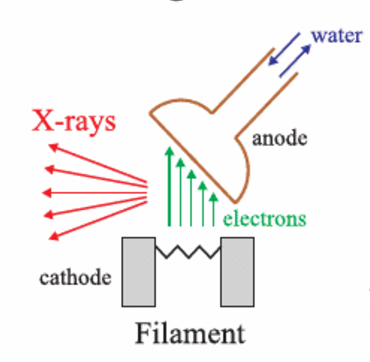
\includegraphics[scale=0.5]{Bilder/tube.png}
    \caption{Schematischer Aufbau einer Röntgenröhre \cite{als-nielsen2011}.}
    \label{fig:roentgenroehre}
\end{figure}

Die Glühkathode emittiert Elektronen durch den glühelektrischen Effekt.
Der glühelektrische Effekt beschreibt die Emission von Elektronen aus einem Festkörper, wenn dieser erhitzt wird.
Die emittierten Elektronen werden durch eine Beschleunigungsspannung $U_\text{B}$ zur Anode hin beschleunigt.
Beim Auftreffen der Elektronen auf die Anode entsteht Röntgenstrahlung \ref{fig:spektrum}.
\begin{figure}[H]
    \centering
    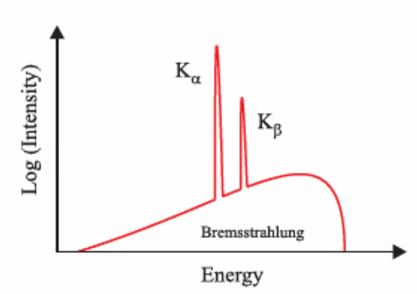
\includegraphics[scale=0.5]{Bilder/spektrum.png}
    \caption{Erzeugte Bremsstrahlung und charakteristische Röntgenstrahlung einer Röntgenröhre \cite{als-nielsen2011}.}
    \label{fig:spektrum}
\end{figure}
Die Röntgenstrahlung setzt sich aus zwei Komponenten zusammen: 
der kontinuierlichen Bremsstrahlung und der charakteristischen Röntgenstrahlung.
Die Bremsstrahlung entsteht, wenn die Elektronen im Coulombfeld der Atomkerne des Anodenmaterials abgebremst werden und dabei Energie verlieren.
Diese Strahlung hat ein kontinuierliches Spektrum, da die Energieabgabe von der Stärke der Abbremsung abhängt.
Die maximale Energie der Bremsstrahlung ist gegeben durch die Beschleunigungsspannung $U_\text{B}$.
Die charakteristische Röntgenstrahlung entsteht, wenn die Elektronen in der Anode in innere Schalen
eines Atoms eindringen und dabei Elektronen aus den Schalen herausschlagen.
Die entstandenen Löcher werden durch Elektronen aus höheren Schalen gefüllt, wobei Röntgenstrahlung emittiert wird.
Die Energie der charakteristischen Röntgenstrahlung ist diskret und entspricht der Energiedifferenz der beteiligten Schalen.
In der Abbildung \ref{fig:spektrum} ist das Spektrum einer Röntgenröhre dargestellt. 
Die $K_\alpha$-Linie entsteht, wenn ein Elektron aus der $L$-Schale in die $K$-Schale fällt, 
während die $K_\beta$-Linie entsteht, wenn ein Elektron aus der $M$-Schale in die $K$-Schale fällt.

\subsection{Röntgenstrahlung an Grenzflächen} \label{sec:reflektivität}
Trifft Röntgenstrahlung auf eine ideal glatte Grenzfläche, 
wie in Abbildung \ref{fig:reflektivität} dargestellt,
gilt für den Brechungsindex $n$ des Mediums
\begin{equation}
    n = 1 - \delta + i\beta,
\end{equation}
wobei $\delta$ und $\beta$ die Dispersion und Absorption des Mediums beschreiben.
\begin{figure}[H]
    \centering
    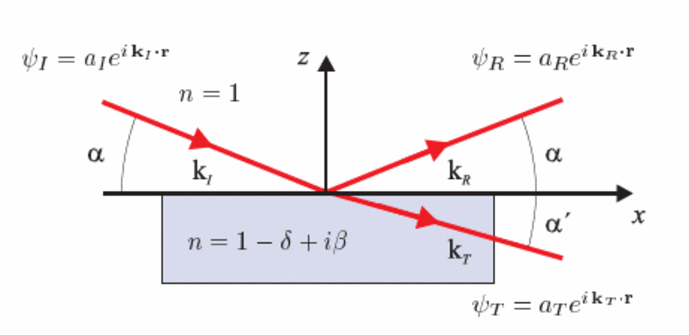
\includegraphics[scale=0.5]{Bilder/reflektion.png}
    \caption{Röntgenstrahlung an einer Grenzfläche \cite{als-nielsen2011}.}
    \label{fig:reflektivität}
\end{figure}
Die Dispersion ist durch die Elektronendichte $\rho$, die Wellenlänge $\lambda$ 
und die Streuamplitude $r_0$ pro Elektron gegeben.
Die Gleichung lautet für die Dispersion lautet
\begin{equation}
    \delta = \frac{r_0 \rho \lambda^2}{2\pi} .
    \label{eq:delta}
\end{equation}
Die Streuamplitude $r_0$ ist gegeben durch die Thomson-Streulänge, 
auch als klassischer Elektronenradius bekannt, und beträgt
\begin{equation}
    r_0 = \SI{2.82e-15}{\meter} .
\end{equation}
Daraus ergibt sich, dass die Dispersion in der Größenordnung von $10^{-6}$ liegt.
Die Absoprtion $\beta$ ist gegeben durch
\begin{equation}
    \beta = \frac{\mu \lambda}{4 \pi} \, ,
    \label{eq:beta}
\end{equation}
wobei $\mu$ der Absorptionskoeffizient ist.
Für die Amplituden der einfallenden, reflektierten und transmittierten Welle gilt
\begin{equation}
    a_I + a_R = a_T 
    \label{eq:amplituden}
\end{equation}
und
\begin{equation}
    a_I \vec{k}_I + a_R \vec{k}_R = a_T \vec{k}_T \, .
\end{equation}
Die Wellenzahl ist im Vakuum gegeben durch $k=|\vec{k}_I| = |\vec{k}_R |$ und im Medium durch $nk = |\vec{k}_T|$.
Für die parallelen und senkrechten Komponenten bezogen auf die Oberfläche der Wellenvektoren gilt
\begin{equation}
    a_I k \cos(\alpha) + a_R k \cos(\alpha) = a_T nk \cos(\alpha') \label{eq:parallel}
\end{equation}
\begin{equation}
    -(a_I-a_R) k \sin(\alpha) = - a_T nk \sin(\alpha') \, . \label{eq:senkrecht}
\end{equation}
Mit den Gleichungen \eqref{eq:amplituden} und \eqref{eq:senkrecht} folgt für kleine Winkel $\alpha$ und $\alpha'$
\begin{equation}
    \frac{a_I-a_R}{a_I+a_R} = n \frac{\sin(\alpha')}{\sin(\alpha)} \approx \frac{\alpha'}{\alpha} \, ,
\end{equation}
woraus sich die Fresnelkoeffizienten
\begin{align}
    r \equiv \frac{a_R}{a_I} &= \frac{\alpha - \alpha'}{\alpha + \alpha'} \, ,\label{eq:fresnel} \\
    t \equiv \frac{a_T}{a_I} &= \frac{2\alpha}{\alpha + \alpha'} \, ,
\end{align}
ergeben.
Für kleine Winkel $\alpha$ und $\alpha'$ und $n\approx1$ kann der Kosinus um Null entwickelt werden, sodass
\begin{equation}
    \label{eq:alpha}
    \alpha' \approx \sqrt{\alpha^2-2\delta} 
\end{equation}
Die Intensität der reflektierten respektive transmittierten Welle ist durch das Betragtsquadrat der Amplitude $r,t$ gegeben.
Der Winkel $\alpha'$, unter dem die transmittierte Welle auftritt, ist eine Komplexezahl und kann in Real- und Imaginärteil
zerlegt werden.
Dabei ist ersichtlich, dass die transmittierte Welle mit zunehmender Tiefe im Medium exponentiell abnimmt.
Die Eindringtiefe ergibt sich somit zu 
\begin{equation}
    \Lambda = \frac{1}{2 k \Im \alpha'} \, \text{with} \, k= \frac{2\pi}{\lambda} \, .
\end{equation}
Bei einem kritischen Winkel $\alpha_c$ tritt Totalreflexion auf, sodass die transmittierte Welle verschwindet.
Der kritischen Winkel ergibt sich durch die Bedingung $\alpha' =0$, einsetzen in das Snellius'sche Brechungsgesetz liefert:
\begin{equation}
   \cos \alpha_c = n \cos \alpha' \quad \Rightarrow \quad \cos \alpha_c = n = 1 - \delta \, .
\end{equation}
Entwicklung des Kosinus um kleine Winkel liefert
\begin{equation}
    \alpha_c \approx \sqrt{2 \delta} \, .
    \label{eq:alpha_c}
\end{equation}
Für Einfallswinkel deutlich größer als $\alpha_c$ ist die Intensität der reflektierten Welle näherungsweise gegeben durch
\begin{equation}
    R = |r|^2 = \left(\frac{\alpha_c}{2 \alpha_I} \right)^4 \, .
    \label{eq:reflektivität_R}
\end{equation}
Das bedeutet, dass die Intensität der reflektierten Welle mit steigendem Einfallswinkel stark abnimmt.
% Seite 79 in Als-Nielsen

\subsection{Multischichtsysteme} \label{sec:multischicht}
Im Gegensatz zu den vorherigen Abschnitten wird nun ein Multischichtsystem betrachtet.
Das Medium, in welches die Röntgenstrahlung eintritt hat folgich keine unendliche Ausdehnung mehr, 
dies ist in Abbildung \ref{fig:multischicht} dargestellt.
\begin{figure}[H]
    \centering
    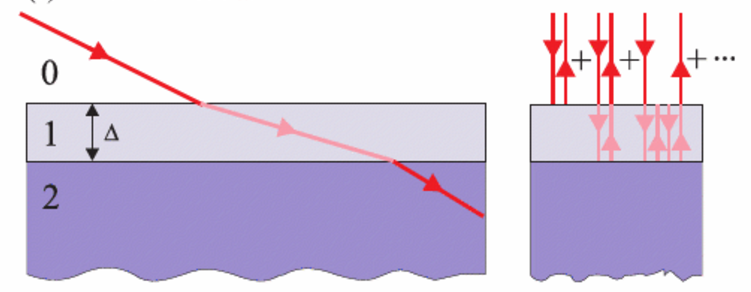
\includegraphics[scale=0.5]{Bilder/multischicht.png}
    \caption{Röntgenstrahlung an einem Multischichtsystem \cite{als-nielsen2011}.}
    \label{fig:multischicht}
\end{figure}
Im Gegensatz zum vorherigen Fall der unendlichen Ausdehnung, gibt es bei eindlicher Ausdehnung, 
wie in Abbildung \ref{fig:multischicht} dargestellt, 
eine unendliche Serie möglicher Reflexionen, wobei die ersten drei dargesteellt sind.
In Abbildung \ref{fig:oszillation} sind die sogenannten Kiessig-Oszillationen dargestellt.
Diese entstehen durch konstruktive und destruktive Interferenz der reflektierten Wellen an den Grenzflächen des Multischichtsystems als Konsequenz der winkelabhängigen Phasenverschiebung.
Die Periode der Oszillationen is gegeben durch die Dicke $d$ der Schicht.
\begin{equation}
    d = \frac{\lambda}{2 \Delta \alpha_I} \, 
    \label{eq:dicke}
\end{equation}
$\Delta \alpha_I$ bezeichnet dabei die Winkeldifferenz zweier Maxima.
\begin{figure}[H]
    \centering
    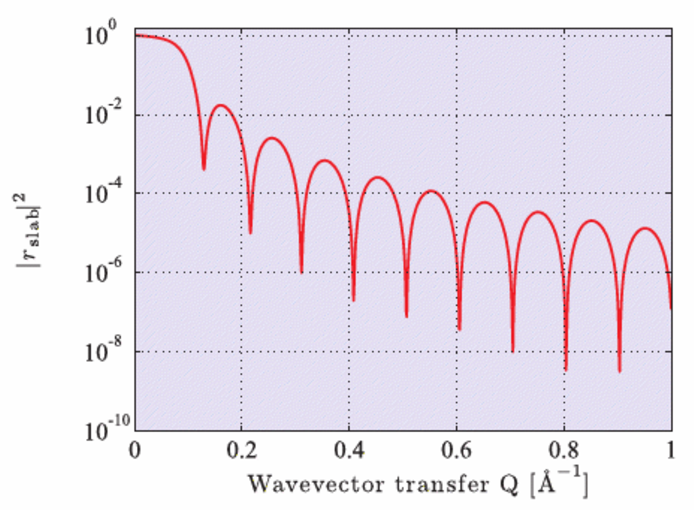
\includegraphics[scale=0.5]{Bilder/oszillation.png}
    \caption{Kiessig-Oszillationen an einem Multischichtsystem \cite{als-nielsen2011}.}
    \label{fig:oszillation}
\end{figure}

% Parratt Algorithmus
\subsubsection{Parratt-Algorithmus} \label{sec:parratt}
Der Parratt-Algorithmus ist ein numerisches Verfahren, um die Reflektivität von Röntgenstrahlung an Multischichtsystemen zu berechnen.
Betrachtet wird ein Medium, bestehend aus $N$ Schichten, wobei die $N$/te Schicht direkt auf dem Substrat liegt.
Das Substrat wird als unendlich dick angesehen.
Jede Schicht des Mediums hat den Brechungsindex $n_j=1-\delta_j+i\beta_j$ mit der Dicke $d_j$.
Das Verhältnis der reflektierten Amplitude $R_{j+1}$ und der transmittierten Amplitude $T_{j+1}$ ist durch $X_{j+1}$ gegeben.
Dadruch lässt sich das Verhältnis der nächsten Schicht mit
\begin{equation}
    X_{j} = \frac{R_j}{T_j} = \exp{(-2i k_{z,j} z_j)} \frac{r_{j,j+1} + X_{j+1} \exp{(2i k_{z,j+1} z_j)}}{1+r_{j,j+1}X_{j+1} \exp{(2i k_{z,j+1} z_j)}}
\end{equation}
bestimmen. Dabei ist $z_j$ die Position der j-ten Schicht und $r_{j,j+1}$ der Fresnelkoeffizient der j-ten Grenzfläche.
Eine schematische Darstellung ist in Abbildung \ref{fig:parratt} zu sehen. 
Es gelten die Randbedingungen $T_1=1$ und $R_{N+1}=0$ und folglich $X_{N+1}=0$ als Start der Rekursion.
\begin{figure}[H]
    \centering
    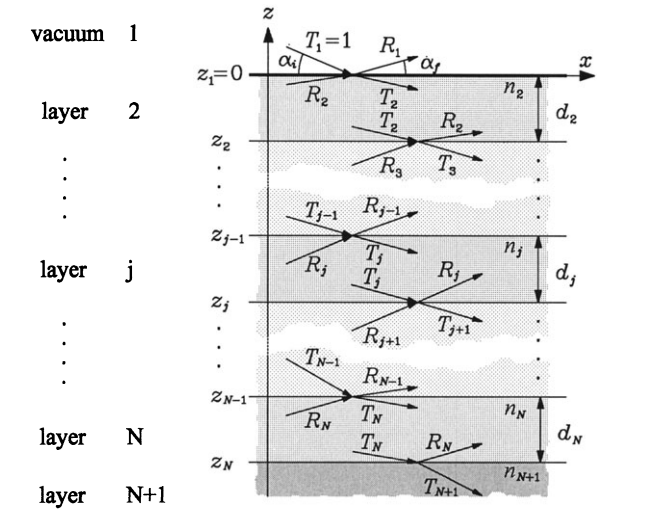
\includegraphics[scale=0.5]{Bilder/parratt.png}
    \caption{Schematische Darstellung eines Mehrschichtsystems mit $N+1$ Schichten und $N$ Grenzflächen \cite{m-tolan2013}.}
    \label{fig:parratt}
\end{figure}
Die z-Komponente des Wellenvektors in der j-ten Schicht ist gegeben durch
\begin{equation}
    k_{z,j} = k \sqrt{n_j^2 - \cos^2\alpha_i} \, ,
\end{equation}
wobei $\alpha_i$ der Einfallswinkel ist.
Für nicht ideal glatte Grenzflächen wird die "root-mean-square" Rauigkeit $\sigma_j$ eingeführt.
Es gilt
\begin{equation}
   \sigma_j^2 = \int (z-z_j)^2 P_j(z) \, \text{d}z \, ,
\end{equation}
wobei $P_j(z)$ die Wahrscheinlichkeitsdichte mit dem Erwartungswert $z_j = \int z P_j(z)\text{d}z$ ist.
Die modifizierten Fresnelkoeffizienten sind gegeben durch
\begin{equation}
    \tilde{r}_{j,j+1} = r_{j,j+1} \exp{(-2 k_{z,j} k_{z,j+1} \sigma_j^2)} \, , \qquad \tilde{t}_{j,j+1} = t_{j,j+1} \exp{((k_{z,j} - k_{z,j+1})^2 \sigma_j^2)/2} \, .
\end{equation}
gegeben. Diese können in den Parratt-Algorithmus eingesetzt werden, um die Reflektivität zu berechnen.

\begin{figure}
    \centering
    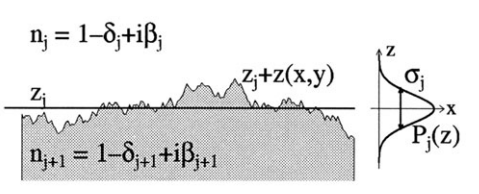
\includegraphics[scale=0.5]{Bilder/sigma.png}
    \caption{Rauigkeit einer Grenzfläche mit der mittleren z-Koordinate $z_j$ und Fluktuation $z(x,y)$. \cite{m-tolan2013}.}
    \label{fig:rauigkeit}
\end{figure}


% Rauigkeit
\subsection{Geometriefaktor} \label{sec:Geometriefaktor}
Unterhalb des Geometriewinkels $\alpha_g$ trifft nicht die gesamte Breite des Strahls die Probe.
Dies wird durch den Geometriefaktor $G$ berücksichtigt.
Der Geometriefaktor ist gegeben durch
\begin{equation}\label{eq:geometriefaktor}
    G = \begin{cases}
        \frac{D \sin(\alpha)}{d} & \text{für} \, \alpha < \alpha_g \\
        1 & \text{für} \, \alpha \geq \alpha_g
    \end{cases} \, ,
\end{equation}
wobei $D$ die Breite der Probe und $d$ die Strahlbreite ist.
Der Geometriewinkel $\alpha_g$ ist gegeben durch
\begin{equation}\label{eq:geometriewinkel}
    \alpha_g = \arcsin \left( \frac{d}{D} \right) \, .
\end{equation}
